% called by main.tex
%
\chapter{Despliegue}
\label{ch::despliegue}

Este capítulo documenta la estrategia de despliegue y, sobre todo, la decisión de no operar
con capital real. El especialista base ofrece una señal fuera de muestra modesta, mientras
que la mejora del filtro de volatilidad procede de un análisis \emph{post-hoc}. El siguiente
paso válido no es producción, sino una sombra prospectiva con la política ya congelada.

\section{Estrategia de despliegue y seguimiento en sombra}

\subsection{Por qué no se despliega}

El resultado limpio se apoya en cinco días, solo tres son positivos y el neto pasa a ser
ligeramente negativo bajo el coste completo. El subconjunto de baja volatilidad es más
prometedor, pero se identificó usando esos mismos cinco días. Desplegar en estas condiciones
confundiría una hipótesis razonable con una validación. Por coherencia con la tesis del
trabajo ---la honestidad del protocolo prevalece sobre cualquier número concreto--- el
proyecto se detiene antes de operar.

\subsection{Del registro retrospectivo a la sombra prospectiva}

El registro disponible es \emph{offline} y retrospectivo: reconstruye, unidad de acción a
unidad de acción, qué habría indicado la regla de baja volatilidad sobre el bloque ya
observado. Sirve para comprobar la contabilidad, el resumen diario y las guardas, pero esos
cinco días no cuentan como validación de la política completa.

A partir del cierre del bloque se congela la regla candidata
($\text{volatilidad}_{5s}\leq0{,}6657$, EV $>0{,}75$ y probabilidad de salud
$\geq0{,}50$). Una sombra prospectiva deberá ejecutarla sin cambios sobre fechas posteriores,
registrar también las abstenciones y resolver la exposición simultánea por mercado. Solo esa
evidencia podrá alimentar las puertas de promoción:

\begin{itemize}[noitemsep]
  \item \textbf{Candidato a seguimiento ampliado:} neto superior a 0,5 ticks, al menos 200
  unidades de acción y al menos 8 días prospectivos.
  \item \textbf{Candidato a despliegue:} neto superior a 0,5 ticks, al menos 400 unidades,
  12 días prospectivos y una regla de exposición/fill validada.
\end{itemize}

En la fecha de corte hay cero días prospectivos de la política completa. Su estado correcto
es \emph{hipótesis congelada pendiente de validación}, no candidata a bot.

\subsection{Diseño de una hipotética API de inferencia}

Solo si se superasen las puertas anteriores, un despliegue eventual tomaría la forma de un
servicio de inferencia con cuatro etapas. Primero, una etapa de ingesta que reconstruyese en
tiempo real el estado del mercado sobre la malla de dos segundos. Segundo, una etapa de
cálculo que generase las 36 características causales del instante actual, idéntica a la del
entrenamiento para evitar discrepancias entre entrenamiento y producción
(\emph{train/serve skew}). Tercero, una etapa de decisión que consultase las dos cabezas del
especialista y devolviese operar o abstenerse. Y cuarto, una capa de guardas que aplicase los
filtros de entorno, volatilidad y obsolescencia, además del límite de exposición por mercado.

Por encima operaría una capa de monitorización que vigilase la deriva de distribución,
registrase cada decisión para auditoría y dispusiese de un interruptor de parada inmediata.
Esta arquitectura es un diseño, no una implementación.

\section{Economía de la ejecución bajo el régimen de comisiones de 2026}

La corrección del modelo de costes (Sección~\ref{sec::fe_erratas_fees}) dejó una
conclusión estructural: el lado \emph{taker} de este mercado no es económico para una
señal de la magnitud encontrada. Pero la misma estructura de comisiones que cierra una
puerta abre otra. Esta sección desarrolla la economía del lado \emph{maker} y el
simulador construido para evaluarla, que es la aportación diferencial del trabajo en el
plano del despliegue.

\subsection{Economía del lado maker y tamaño del premio}

Quien cruza el mercado (\emph{taker}) paga una comisión $C\cdot r\cdot p\,(1-p)$; quien
aporta liquidez (\emph{maker}) está exento y, además, recibe una parte del fondo de
comisiones en forma de \emph{rebate}, aproximadamente el 20\,\% del fondo repartido con el
mismo peso $p\,(1-p)$. Ese peso (Figura~\ref{fig::pq}) concentra tanto la comisión como el
reparto en torno a $p=0{,}5$ —la zona de precios donde opera este trabajo— y se anula en
los extremos, cerca de la resolución. El vehículo económico se invierte respecto al taker:
donde uno paga el \emph{spread} y la comisión, el otro los cobra.

\begin{figure}[htbp]
\centering
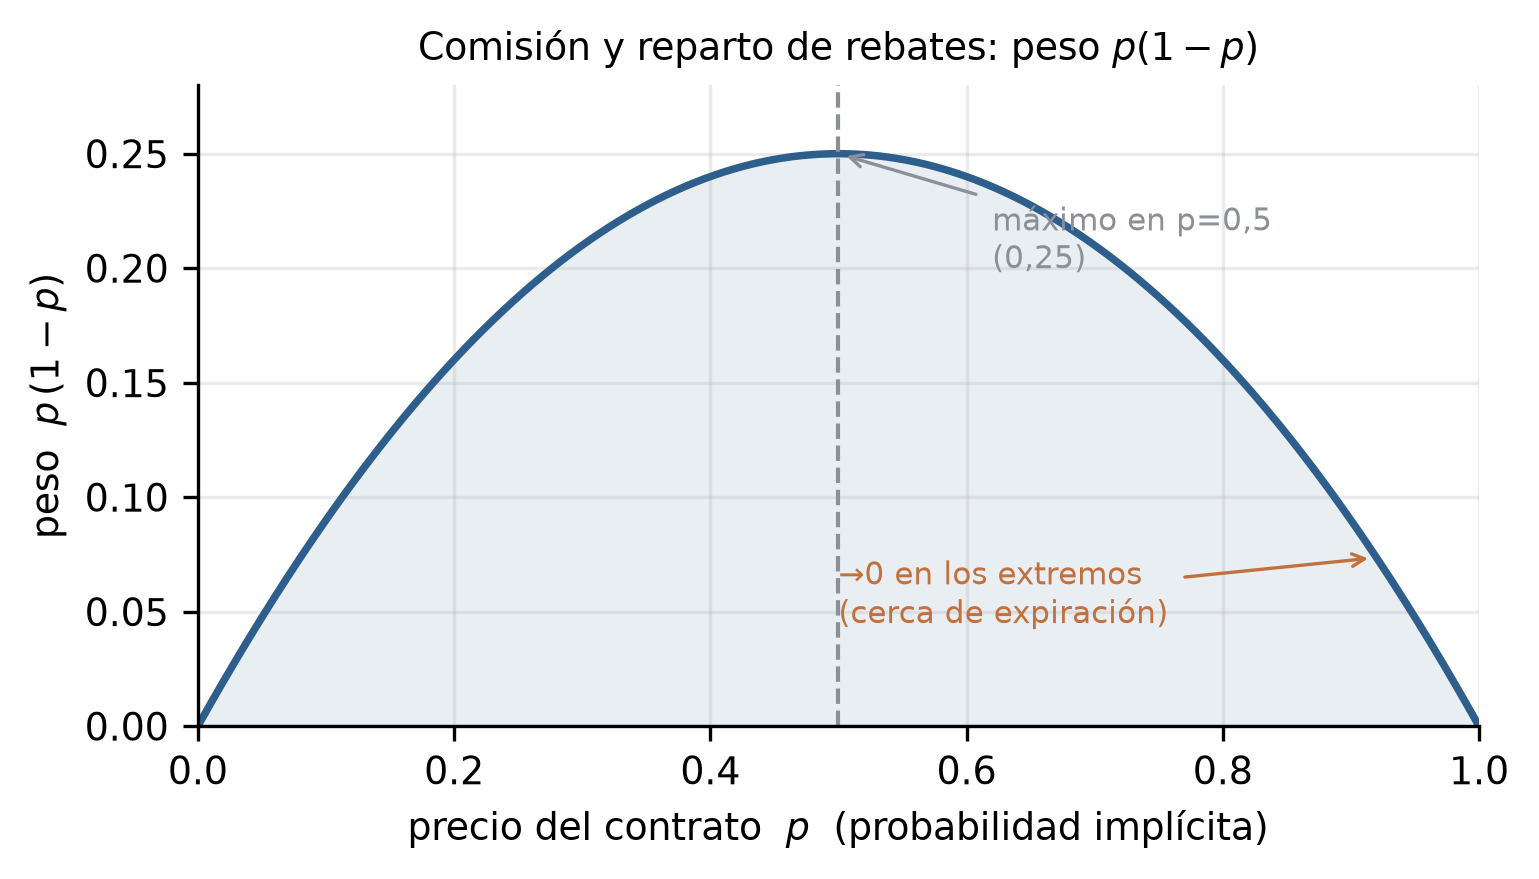
\includegraphics[width=0.62\textwidth]{figures/fig_pq_weight.png}
\caption{El peso $p\,(1-p)$ que gobierna la comisión taker y el reparto de \emph{rebates}
al maker: máximo en $p=0{,}5$ y nulo en los extremos. La economía maker es más densa
precisamente en la zona de precios intermedios donde opera el trabajo.}
\label{fig::pq}
\end{figure}

El tamaño del premio se midió sobre la copia histórica (solo lectura) antes de construir
nada. El universo de mercados horarios de Bitcoin mueve del orden de
\$310.000 de nocional al día (\$434.000 contando todas las temporalidades), con una
concentración baja —el 10\,\% de mercados más grandes reúne solo el 23\,\% del volumen— y
una distribución horaria plana: no hay «mercado estrella» ni «hora mágica» por los que
competir, de modo que la ventaja está en la presencia continua, que la infraestructura
24/7 del proyecto ya proporciona. El fondo de \emph{rebates} resultante se estima entre
\$1.100 y \$3.000 al día, entre diez y veinte veces por encima del umbral por debajo del
cual la vía se habría descartado por insignificante. La puerta económica del lado maker,
por tanto, se pasa con holgura —a diferencia de la taker.

\subsection{El simulador de colas y \emph{fills}}
\label{sec::simulador_maker}

Para evaluar la vía maker sin operar con dinero se construyó un simulador de ejecución
sobre el libro L2 agregado a 2 segundos y la cinta de operaciones capturada, con las
reglas del \emph{venue} separadas del motor para poder auditarlas y reutilizarlas. La
estrategia base se une al mejor precio de compra y de venta sin mejorarlo, con tamaño
fijo, solo cuando el \emph{spread} alcanza un mínimo, y con un tope de inventario; recotiza
cuando el mejor nivel se mueve, perdiendo su lugar en la cola.

El modelo de \emph{fill} es deliberadamente conservador donde puede y explícito en sus
sesgos donde no. La cola por delante al colocar una orden se fija en todo el tamaño
visible del nivel (se asume que todos los demás llegaron antes); el flujo \emph{taker} de
cada frame consume cola cuando la última operación ocurrió a nuestro precio, y un barrido
más allá del precio produce ejecución completa. Sin datos de nivel 3 no existe una verdad
de cola, por lo que el simulador se declara una \emph{cota}, no una medida: su sesgo
optimista (atribuir todo el flujo del frame a nuestro nivel) y su sesgo pesimista (no
adelantar a nadie tras recotizar) se netean en la calibración pendiente contra la cinta
fresca. La economía por sesión se contabiliza como caja más inventario valorado a la
resolución más \emph{rebates}; el \textbf{riesgo terminal binario} está incluido: el
inventario que queda al expirar liquida a 0 o a 1 según el desenlace del mercado.

El resultado más informativo del simulador no es el número —una banda de entre \$25 y
\$200 diarios de beneficio bruto simulado según régimen y configuración, cuyo signo
sobrevive a los ajustes estrictos— sino la \emph{descomposición} del riesgo. La selección
adversa medida por el \emph{markout} a corto plazo es \textbf{favorable} (alrededor de
$+1$ tick): estos libros revierten a pocos segundos, y esa misma predictibilidad de corto
plazo que el taker no podía pagar por culpa de la comisión es la que cobra el maker
pasivo. El coste no está ahí, sino en el \textbf{inventario retenido hasta la
expiración}, que resuelve en contra —la selección adversa vive en el tramo terminal, no en
el \emph{markout} corto—. La consecuencia de diseño es directa y conecta con la
Sección~\ref{sec::tramo_terminal}: la palanca dominante es el control de inventario
—aplanar la posición antes del tramo en que el precio se decide—, no la captura de
\emph{spread} en sí. Introducir una zona plana en los últimos minutos, cotizando solo el
lado que reduce inventario, es lo que separa un simulador que pierde en el terminal de uno
que conserva el signo.

Las reservas de esta evaluación se declaran sin adornos. El modelo de \emph{fill} es una
cota superior; los lados \textsc{sí} y \textsc{no} del mismo mercado se tratan como riesgos
independientes cuando en realidad están correlacionados; el corpus es de mayo a junio, sin
validación prospectiva; y, sobre todo, ningún \emph{replay} histórico puede capturar la
respuesta competitiva de los creadores de mercado incumbentes
(Capítulo~\ref{ch::etica}), lo que sitúa la banda simulada como optimista. Es evidencia
suficiente para justificar la validación prospectiva pre-registrada, no para afirmar
rentabilidad.

\subsection{El tramo terminal: cuándo el precio se vuelve informativo}
\label{sec::tramo_terminal}

El riesgo central de un creador de mercado en estos contratos no está en el
\emph{spread} que cobra, sino en el inventario que le queda cuando el mercado resuelve:
un contrato binario liquida a 0 o a 1, de modo que una posición sin cerrar a la
expiración se enfrenta a una varianza estructural de settlement. Para dimensionar ese
riesgo hace falta saber \emph{cuándo} el precio deja de ser una moneda al aire sobre el
desenlace. Se mide de forma directa —sin entrenar ningún modelo, como baseline previo a
cualquier modelo secuencial— tratando el precio medio como estimador de la probabilidad
de settlement y evaluando su calibración a lo largo de la vida del mercado con
\emph{proper scoring} (puntuación de Brier) por tiempo a expiración. La etiqueta es el
settlement real, aproximado por el precio medio del último frame observado cuando este
cae a menos de cinco minutos del cierre y ha convergido a 0 o 1; las series cuyo último
frame queda lejos del cierre se censuran. El universo etiquetado (310 series, con
balance exacto entre desenlaces) es un subconjunto sesgado del corpus —el observado
cerca del cierre—, lo que se declara como limitación.

El resultado (Figura~\ref{fig::n1}, panel izquierdo) es una caída suave y monótona de la
puntuación de Brier: en la apertura del mercado (50--60 minutos a expiración) vale
$0{,}234$, apenas por debajo del $0{,}25$ de la moneda al aire, y el acierto direccional
sobre el desenlace es del 58\,\%; el precio no se vuelve claramente informativo hasta los
últimos quince a veinte minutos, donde la puntuación cae por debajo de $0{,}10$ (acierto
del 90\,\% o más) y, en el último minuto, converge al settlement. Dicho de otro modo, durante
la mayor parte de la vida del contrato el precio medio de Polymarket es honesto pero poco
resolutivo, y toda la información se concentra en el tramo final.

El panel derecho matiza el diagnóstico con curvas de fiabilidad en dos cortes. Lejos del
cierre, el precio está \emph{bien calibrado} —un precio de $0{,}25$ resuelve a favor en
un 31\,\% de los casos y uno de $0{,}75$ en un 69\,\%, cerca de la diagonal— pero con casi
toda su masa concentrada en torno a $0{,}5$: el mercado dice correctamente «no lo sé». Al
acercarse el cierre, la distribución se polariza hacia 0 y 1 conforme llega la
información, manteniendo la calibración en los extremos. La consecuencia para el diseño
maker es inmediata: el precio sirve como probabilidad (no hay que corregir su sesgo), pero
la ventana en la que el inventario deja de ser una apuesta y pasa a estar decidido es
estrecha y tardía, lo que convierte el aplanado de inventario \emph{antes} de ese tramo en
la palanca de riesgo dominante del simulador —coherente con la concentración de actividad
en el minuto 50 detectada en el análisis exploratorio (Sección~\ref{sec::eda_series}).

\begin{figure}[htbp]
\centering
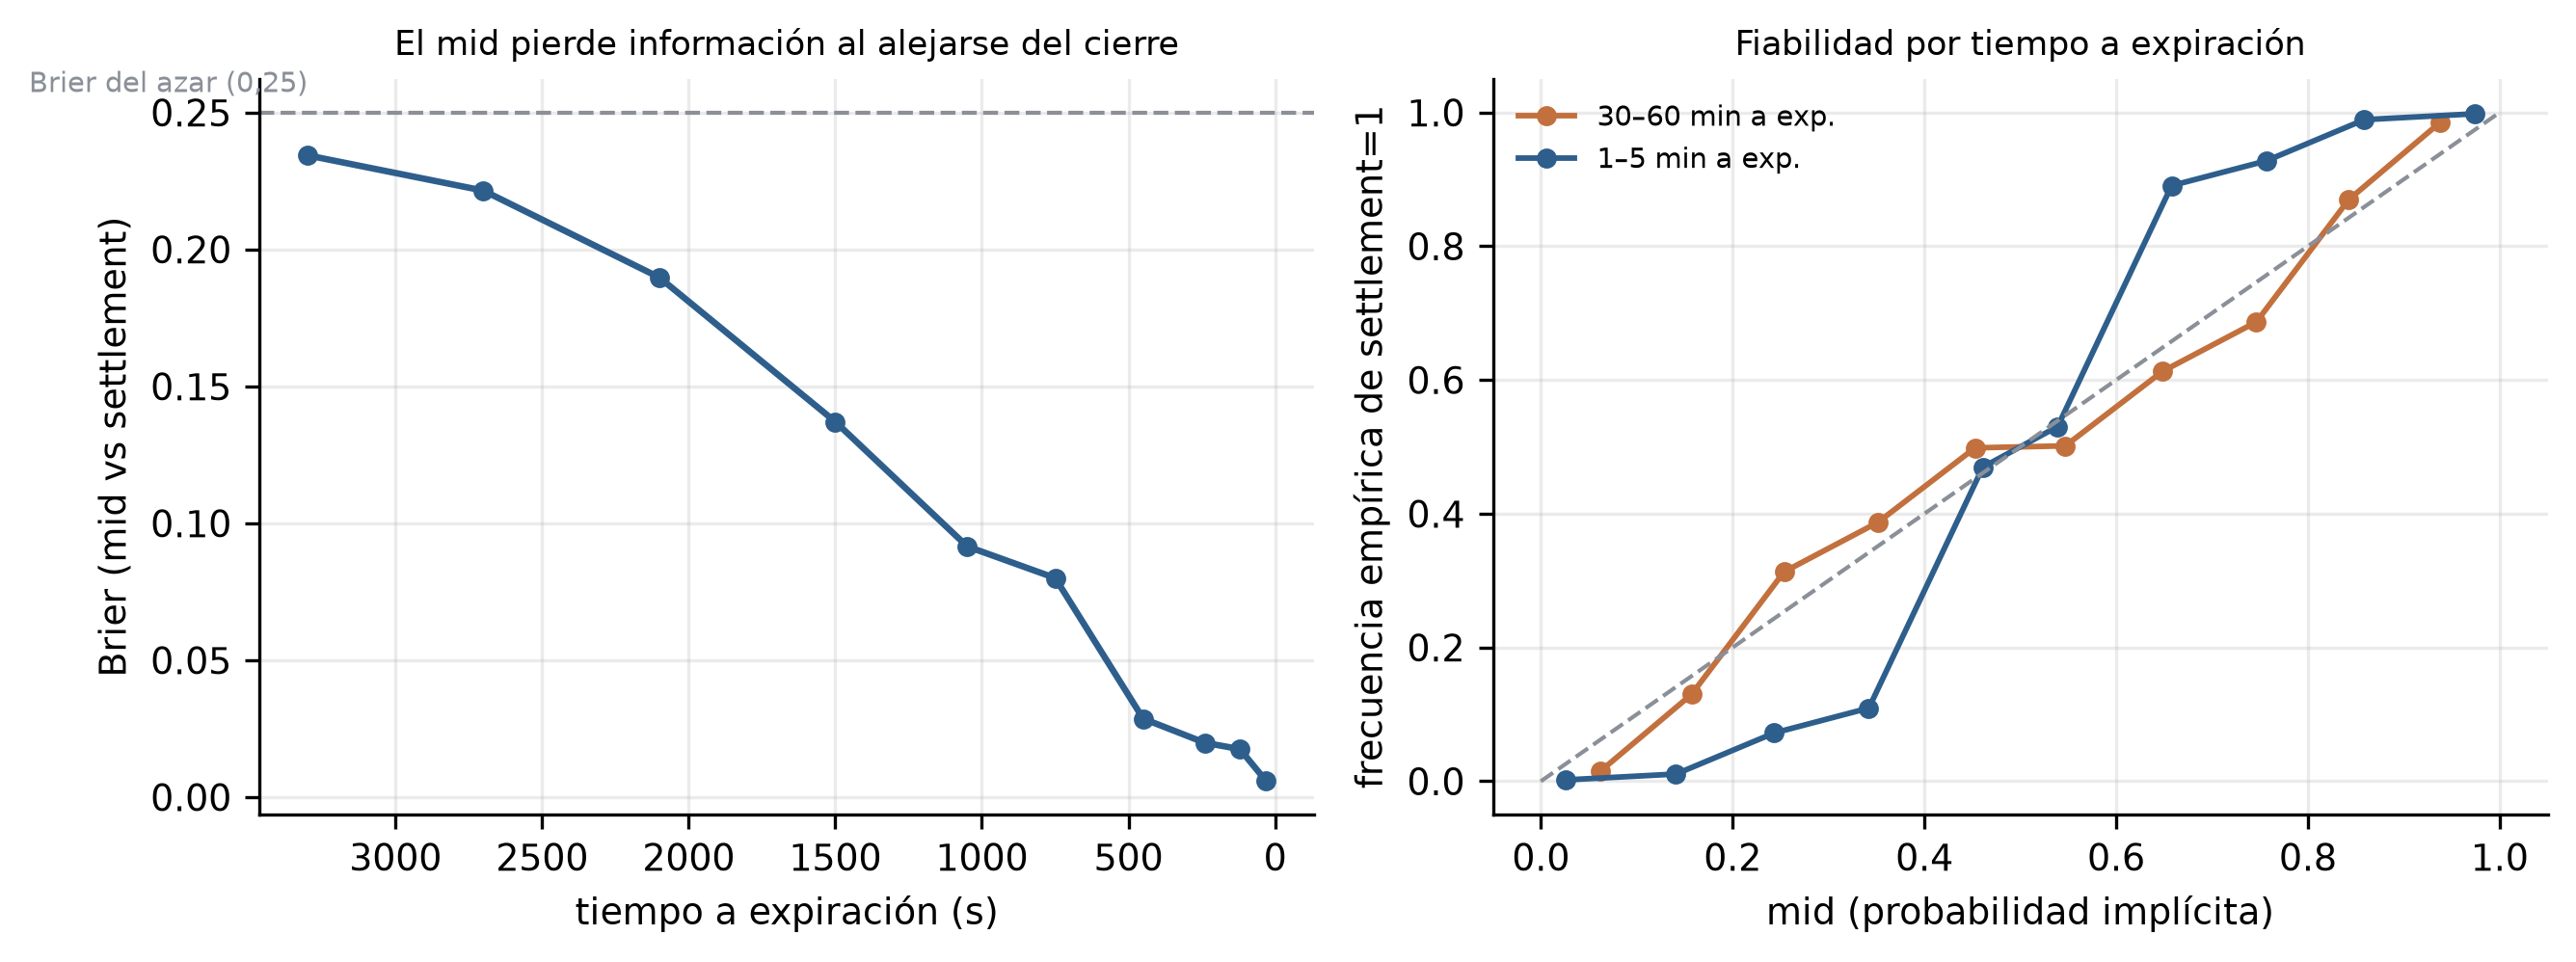
\includegraphics[width=\textwidth]{figures/fig_n1_calibracion_terminal.png}
\caption{Informatividad del precio medio sobre el settlement. Izquierda: puntuación de
Brier por tiempo a expiración; el precio es casi una moneda al aire en la apertura y solo
se vuelve informativo en el tramo terminal. Derecha: curvas de fiabilidad lejos (30--60
min) y cerca (1--5 min) del cierre; el precio está bien calibrado en ambos cortes, pero
su masa se polariza al acercarse la expiración.}
\label{fig::n1}
\end{figure}

Cabe preguntarse si un modelo aprendido extraería la señal del desenlace \emph{antes}
que el precio, a partir de la microestructura (\emph{imbalance}, flujo de órdenes,
presión del libro). Se comprobó de forma directa, como paso previo a cualquier modelo
secuencial: un \emph{gradient boosting} sobre esas características, con partición temporal
estricta (entrenamiento en mayo, prueba en junio, agrupando por mercado), no mejora la
puntuación de Brier del propio precio (0,141 frente a 0,140) en ningún tramo de tiempo a
expiración; usando \emph{solo} el flujo, sin el precio, la puntuación es peor (0,20) y a
tiempo a expiración grande cae al azar. La microestructura no aporta información sobre el
settlement que el precio no capture ya: a este horizonte, el precio es prácticamente un
estadístico suficiente. En consecuencia no se entrena un modelo secuencial dedicado
—sobre apenas un centenar de desenlaces independientes solo añadiría riesgo de
sobreajuste—, y la curva de Brier por tiempo a expiración se emplea directamente como
cronograma de aplanado de inventario en el simulador.
